\chapter{Bài 7. Gia tốc - Chuyển động thẳng biến đổi đều }
\begin{center}
\itshape (4 tiết)
\end{center}
\section{MỤC TIÊU DẠY HỌC}
\begin{center}
	\begin{longtable}{|M{2.5cm}|L{12.5cm}|M{2cm}|}
		\hline
		\thead{Biểu hiện\\ năng lực} & \thead{Mục tiêu} & \thead{STT}\\
		\hline
		\multicolumn{3}{|c|}{\textbf{ Năng lực vật lí}}\\
		\hline
		1.1 & Lập luận dựa vào sự biến đổi vận tốc trong chuyển động thẳng, rút ra được công thức tính gia tốc.  & 1\\
		\hline
		1.1 & Nêu được ý nghĩa, đơn vị của gia tốc.  & 2\\
		\hline
		1.2 & Dựa trên số liệu cho trước vẽ được đồ thị vận tốc – thời gian trong chuyển động thẳng. & 3\\
		\hline
		1.2 & Vận dụng đồ thị vận tốc – thời gian để tính được độ dịch chuyển và gia tốc trong một số trường hợp đơn giản. & 4\\
		\hline
		1.2 & Rút ra được các công thức của chuyển động thẳng biến đổi đều (không được dùng tích phân). & 5\\
		\hline
		1.2 & Vận dụng được các công thức của chuyển động thẳng biến đổi đều. & 6\\
		\hline
		\multicolumn{3}{|c|}{\textbf{Năng lực chung}}\\
		\hline
		GT - HT & Chủ động trong giao tiếp khi làm việc nhóm; biết khiêm tốn tiếp thu sự góp ý và nhiệt tình chia sẻ, hỗ trợ các thành viên trong nhóm. & 7\\
		\hline
		TC - TH & Chủ động, tích cực thực hiện các nhiệm vụ được đặt ra cho các nhóm; tự điều chỉnh thái độ, hành vi của bản thân, bình tĩnh và có cách cư xử đúng khi giao tiếp trong quá trình làm việc nhóm. & 8\\
		\hline
	\end{longtable}
\end{center}
\section{THIẾT BỊ DẠY HỌC VÀ HỌC LIỆU}
\begin{itemize}
	\item Tivi/máy chiếu.
	\item Phiếu thảo luận nhóm.
\end{itemize}
\section{TIẾN TRÌNH DẠY HỌC}
\subsection{TIẾN TRÌNH}
\begin{center}
	\begin{longtable}{|L{2.75cm}|C{1.25cm}|L{5cm}|L{3.5cm}|L{4cm}|}
		\hline
		\thead{Tiến trình} & \thead{Mục\\tiêu} & \thead{Nội dung dạy học \\trọng tâm} & \thead{PP,\\ KTDH} & \thead{Phương pháp \\đánh giá}\\
		\hline
		\textbf{Hoạt động 1:} Tìm hiểu khái niệm và ý nghĩa của gia tốc. & 1, 2, 7, 8 & Công thức tính gia tốc, ý nghĩa và đơn vị của gia tốc.&PP: Dạy học giải quyết vấn đề, thuyết trình. & GV đánh giá dựa trên kết quả báo cáo thảo luận nhóm của HS.\newline
		PP đánh giá: quan sát, nghe.\\
		\hline
		\textbf{Hoạt động 2:} Vận dụng đồ thị vận tốc – thời gian để tính độ dịch chuyển và gia tốc. & 3, 4, 7, 8 & Đồ thị vận tốc – thời gian trong chuyển động thẳng biến đổi đều.\newline
		Vận dụng đồ thị vận tốc – thời gian để tính độ dịch chuyển và gia tốc trong trường hợp đơn giản.
		& PP dạy học: Dạy học hợp tác, thuyết trình.\newline
		KTDH: Chia sẻ cặp đôi.
		& GV đánh giá dựa trên kết quả trên phiếu học tập và bài báo cáo của nhóm HS.\newline
		PP đánh giá: quan sát, nghe.\\
		\hline
		\textbf{Hoạt động 3:} Rút ra các công thức của chuyển động thẳng biến đổi đều. & 5, 7, 8 & Các công thức chuyển động thẳng biến đổi đều. & PP: Dạy học hợp tác. & GV đánh giá dựa trên kết quả hoạt động nhóm của HS trên phiếu học tập.\newline
		PP đánh giá: quan sát, nghe.\\
		\hline
		\textbf{Hoạt động 4:} Luyện tập. & 3, 4, 6 & Vận dụng các công thức chuyển động thẳng biến đổi đều. & PP: Đàm thoại & GV đánh giá dựa trên bài tập cá nhân của HS.\newline
		PP đánh giá: quan sát.\\
		\hline
	\end{longtable}
\end{center}
\subsection{CÁC HOẠT ĐỘNG HỌC}
\hoatdong{
Tìm hiểu khái niệm và ý nghĩa của gia tốc
}
{HS rút ra được công thức tính gia tốc.
	
HS nêu được ý nghĩa và đơn vị của gia tốc.
}
{
Phiếu hoạt động nhóm số 1 + Phần trình bày của nhóm HS.
}
{
\textit{\underline{* GV chuyển giao nhiệm vụ học tập}}\\
GV chia lớp thành 4 nhóm. GV yêu cầu HS đọc kĩ nhiệm vụ của hoạt động 1 và thảo luận theo nhóm đã chia. Sau 10 phút, GV gọi 1 nhóm lên trình bày kết quả thảo luận của nhóm, các nhóm còn lại góp ý/bổ sung.\\
\textit{\underline{* HS thực hiện nhiệm vụ học tập}}\\
HS \textit{(làm việc theo nhóm)}: Tiến hành thảo luận, đưa ra đáp án + lời giải thích cho mỗi tình huống trong phiếu học tập số 1. Nhóm HS trình bày kết quả vào phiếu học tập và thống nhất chọn đại diện báo cáo.\\
GV: Theo dõi các nhóm thảo luận để phát hiện kịp thời vấn đề mà nhóm HS gặp phải, từ đó đưa ra sự định hướng, hỗ trợ phù hợp cho mỗi nhóm.\\
\textit{\underline{* HS báo cáo kết quả thực hiện nhiệm vụ học tập}}\\
GV: Yêu cầu đại diện của 1 nhóm HS lên trình bày kết quả hoạt động 1. Các nhóm còn lại chú ý theo dõi để nhận xét.

HS: Đặt câu hỏi, góp ý.

GV: Chỉnh lí, hợp thức hoá kiến thức.

GV: Từ kết quả báo cáo của HS, GV giới thiệu khái niệm và ý nghĩa của gia tốc.

HS: Ghi chép nội dung trọng tâm vào vở.
}
%%%%%%%%%%%%%%%%%%%%%%%%%%%%%%%%%%%%%%%%%%%%%%%%%%%%%%%%%%%%%%%
\hoatdong{
Vận dụng đồ thị vận tốc – thời gian để tính độ dịch chuyển và gia tốc
}
{
	HS vận dụng đồ thị vận tốc – thời gian để tính được độ dịch chuyển và gia tốc trong một số trường hợp đơn giản.
}
{
Phiếu hoạt động nhóm số 2 + Phần trình bày của HS.
}
{
\textit{\underline{GV chuyển giao nhiệm vụ học tập}}\\
GV hướng dẫn HS cách xác định độ dịch chuyển từ đồ thị vận tốc – thời gian.

GV chia lớp thành các nhóm đôi. Một nửa số nhóm thực hiện câu a, các nhóm còn lại thực hiện câu b. 

GV yêu cầu HS đọc kĩ nhiệm vụ của hoạt động 2 và thảo luận theo nhóm đã chia. Sau 10 phút, GV gọi 2 HS đại diện của 2 nhóm lên trình bày kết quả hoạt động, các nhóm còn lại góp ý/bổ sung.\\
\textit{\underline{HS thực hiện nhiệm vụ học tập}}\\
HS \textit{(làm việc theo nhóm đôi)}: Tiến hành thảo luận, đưa ra đáp án trong phiếu học tập số 2. 

GV: Theo dõi để phát hiện các HS gặp khó khăn, từ đó đưa ra sự định hướng, hỗ trợ phù hợp cho mỗi HS.\\
\textit{\underline{HS báo cáo kết quả thực hiện nhiệm vụ học tập}}\\
GV: Yêu cầu đại diện của 2 nhóm HS lên trình bày kết quả hoạt động 2. Các nhóm còn lại chú ý theo dõi để nhận xét.

HS: Đặt câu hỏi, góp ý.

GV: Chỉnh lí, hợp thức hoá kiến thức.


}
%%%%%%%%%%%%%%%%%%%%%%%%%%%%%%%%%%%%%%%%%%%%%%%%%%%%%%%%%%%
\hoatdong{
Rút ra các công thức của chuyển động thẳng biến đổi đều.
}
{
HS vận dụng đồ thị vận tốc – thời gian để rút ra công thức tính độ dịch chuyển trong chuyển động thẳng biến đổi đều.
}
{
	Phiếu hoạt động nhóm số 3 + Phần trình bày của HS.
}
{
\textit{\underline{* GV chuyển giao nhiệm vụ học tập}}\\
GV yêu cầu HS hoạt động theo nhóm lớn đã chia và đọc kĩ nhiệm vụ của hoạt động 3. Sau 10 phút, GV gọi 1 HS đại diện của 1 nhóm lên trình bày kết quả hoạt động, các nhóm còn lại góp ý/bổ sung.\\
\textit{\underline{* HS thực hiện nhiệm vụ học tập}}
HS (làm việc theo nhóm lớn): Tiến hành thảo luận, đưa ra đáp án trong phiếu học tập số 3. 

GV: Theo dõi để phát hiện các HS gặp khó khăn, từ đó đưa ra sự định hướng, hỗ trợ phù hợp cho mỗi HS.\\
\textit{\underline{* HS báo cáo kết quả thực hiện nhiệm vụ học tập}}\\
GV: Yêu cầu đại diện của 1 nhóm HS lên trình bày kết quả hoạt động 3. Các nhóm còn lại chú ý theo dõi để nhận xét.

HS: Đặt câu hỏi, góp ý.

GV: Chỉnh lí, hợp thức hoá kiến thức.
}
%%%%%%%%%%%%%%%%%%%%%%%%%%%%%%%%%%%%%%%%%%%%%
\hoatdong{
Luyện tập.
}
{
HS vận dụng được các công thức của chuyển động thẳng biến đổi đều.
}
{
Bài tập cá nhân của học sinh.
}
{
\textit{\underline{* GV chuyển giao nhiệm vụ học tập}}\\
GV lần lượt chuyển giao từng bài tập, yêu cầu HS hoạt động cá nhân để giải.\\
\textit{\underline{* HS thực hiện nhiệm vụ học tập}}\\
HS \textit{(làm việc cá nhân)}:  Giải bài tập trong phiếu bài tập được GV giao. 

GV: Theo dõi để phát hiện các HS gặp khó khăn, từ đó đưa ra sự định hướng, hỗ trợ phù hợp cho mỗi HS.\\
\textit{\underline{* HS báo cáo kết quả thực hiện nhiệm vụ học tập}}\\
GV: Mời HS lên bảng giải bài tập.

HS: Đặt câu hỏi, góp ý.

GV: Chỉnh lí, hợp thức hoá kiến thức.
}

\section{HỒ SƠ DẠY HỌC}
\subsection{NỘI DUNG DẠY HỌC}
\begin{enumerate}[label=\bfseries\arabic*.]
	\item \textbf{Gia tốc}\\
	Gia tốc là đại lượng đặc trưng cho độ biến thiên của vận tốc theo thời gian. Trong chuyển động thẳng, gia tốc trung bình được xác định theo biểu thức:
	\begin{equation}
		a_{tb}=\dfrac{\Delta v}{\Delta t}=\dfrac{v-v_0}{\Delta t}
	\end{equation}
	Trong hệ SI, đơn vị của gia tốc là $\si{\meter/\second^2}$.\\
	Khi $\Delta t$ rất nhỏ, gia tốc trung bình trở thành gia tốc tức thời. Gia tốc tức thời tại một thời điểm có giá trị bằng độ dốc của tiếp tuyến của đồ thị vận tốc – thời gian.\\
	Dựa vào gia tốc tức thời, ta có thể phân chuyển động thẳng thành 3 loại:
	\begin{center}
		\begin{tabular}{|M{5cm}|M{5cm}|M{6cm}|}
			\hline
			Chuyển động thẳng đều & Chuyển động thẳng biến đổi đều & Chuyển động thẳng biến đổi phức tạp\\
			\hline
			$a=0$ & $a=const\neq0$ & $a\neq0$ nhưng không phải hằng số\\
			\hline
		\end{tabular}
	\end{center}
	\item \textbf{Đồ thị vận tốc - thời gian}\\
	\begin{enumerate}[label=\bfseries \itshape 2.\arabic*., nolistsep]
		\item  \textbf{\textit{Đồ thị vận tốc – thời gian của chuyển động thẳng biến đổi đều}}\\
		Chuyển động thẳng biến đổi đều là chuyển động thẳng mà vận tốc có độ lớn tăng đều hoặc giảm đều theo thời gian:
		\begin{itemize}
			\item chuyển động thẳng có độ lớn vận tốc tăng đều theo thời gian gọi là chuyển động thẳng nhanh dần đều ( $\vec{a}\uparrow\uparrow\vec{v}$ hay $a\cdot v>0$);
			\item chuyển động thẳng có độ lớn vận tốc giảm dần theo thời gian gọi là chuyển động thẳng chậm dần đều ($\vec{a}\uparrow\downarrow\vec{v}$  hay  $a\cdot v<0$).
			
		\end{itemize}
		Nếu tại thời điểm $t_0=0$   vật có vận tốc $v_0$ thì phương trình vận tốc của vật tại thời điểm $t$:
		\begin{equation}
			v=v_0+at
		\end{equation}
		Đồ thị vận tốc – thời gian của vật chuyển động thẳng biến đổi đều có dạng:
		\begin{center}
			\begin{tabular}{M{8.5cm}M{8.5cm}}
				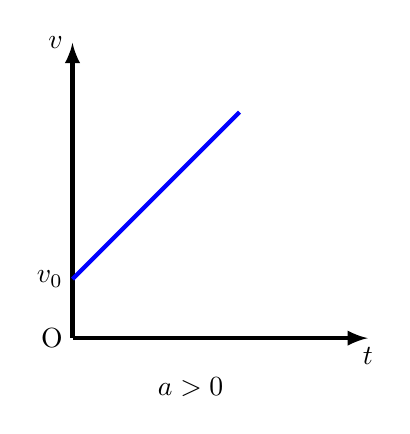
\begin{tikzpicture}[scale=0.75]  
					\coordinate (O) at(0,0);
					\coordinate (x) at(5,0);
					\coordinate (y) at(0,5);
					\coordinate (v0) at(0,1);
					\draw[-latex, line width=1.5pt] (O)--(x);
					\draw[-latex, line width=1.5pt] (O)--(y);
					\draw[blue, line width=1.5pt] (v0)--+(45:4);
					\node[below] at(x) {$t$};
					\node[left] at(y) {$v$};
					\node[left] at(v0) {$v_0$};
					\node[left] at(O) {O};
					\node[below] at (2,-0.5) {$a>0$};
				\end{tikzpicture}
				&
				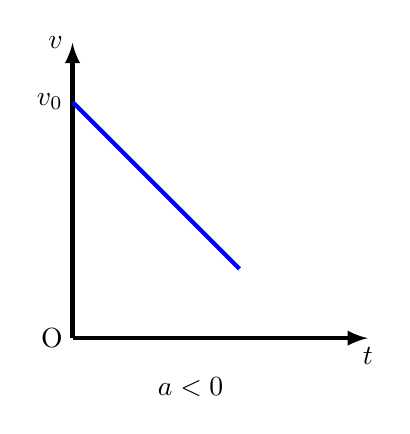
\begin{tikzpicture}  [scale=0.75] 
					\coordinate (O) at(0,0);
					\coordinate (x) at(5,0);
					\coordinate (y) at(0,5);
					\coordinate (v0) at(0,4);
					\draw[-latex, line width=1.5pt] (O)--(x);
					\draw[-latex, line width=1.5pt] (O)--(y);
					\draw[blue, line width=1.5pt] (v0)--+(-45:4);
					\node[below] at(x) {$t$};
					\node[left] at(y) {$v$};
					\node[left] at(v0) {$v_0$};
					\node[left] at(O) {O};
					\node[below] at (2,-0.5) {$a<0$};
				\end{tikzpicture}
			\end{tabular}
		\end{center}
		\item \textbf{\textit{Vận dụng độ thị vận tốc – thời gian để tính độ dịch chuyển}}\\
		\begin{center}
			\begin{tabular}{M{8cm}M{8cm}}
				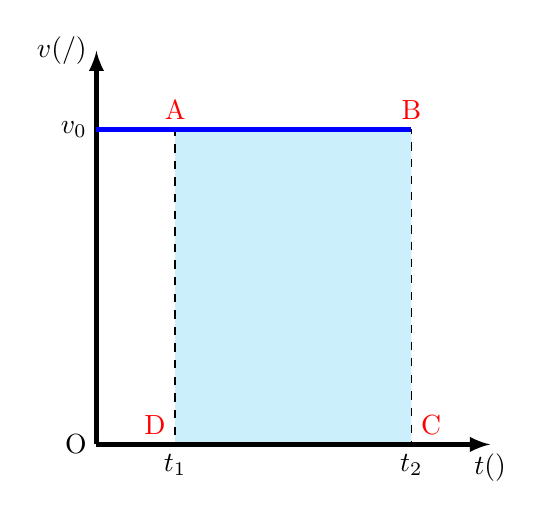
\begin{tikzpicture}  
					\coordinate (O) at(0,0);
					\coordinate (x) at(5,0);
					\coordinate (y) at(0,5);
					\coordinate (v0) at(0,4);
					\coordinate (A) at(1,4);
					\coordinate (B) at(4,4);
					\coordinate (C) at(4,0);
					\coordinate (D) at(1,0);
					\draw[-latex, line width=1.5pt] (O)--(y);
					\fill[cyan, opacity=0.2] (A)--(B)--(C)--(D)--(A);
					\draw[line width=0.5pt,black, dashed] (A)--(B)--(C)--(D)--(A);
					\draw[-latex, line width=1.5pt] (O)--(x);
					\draw[blue, line width=1.5pt] (v0)--(B);
					\node[below] at(x) {$\xsi{t}{\left(\second\right)}$};
					\node[left] at(y) {$\xsi{v}{(\meter/\second)}$};
					\node[left] at(v0) {$v_0$};
					\node[left] at(O) {O};
					\node[below] at (C) {$t_2$};
					\node[below] at (D) {$t_1$};
					\node[above, red] at(A) {A};
					\node[above, red] at(B) {B};
					\node[above right, red] at(C) {C};
					\node[above left, red] at(D) {D};
				\end{tikzpicture}
				&
				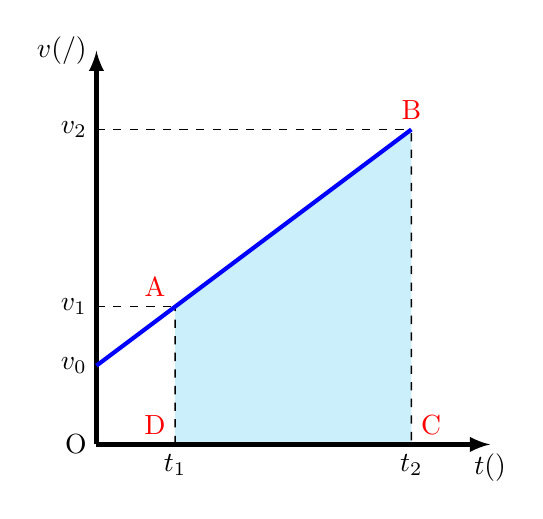
\begin{tikzpicture}  
					\coordinate (O) at(0,0);
					\coordinate (x) at(5,0);
					\coordinate (y) at(0,5);
					\coordinate (v0) at(0,1);
					\coordinate (v1) at(0,1.75);
					\coordinate (v2) at(0,4);
					\coordinate (B) at(4,4);
					\coordinate (A) at(1,1.75);
					\coordinate (C) at(4,0);
					\coordinate (D) at(1,0);
					\fill[cyan, opacity=0.2] (A)--(B)--(C)--(D)--(A);
					\draw[line width=0.5pt,black, dashed] (A)--(B)--(C)--(D)--(A);
					\draw[line width=0.5pt, dashed] (v1)--(A);
					\draw[line width=0.5pt, dashed] (v2)--(B);
					\draw[-latex, line width=1.5pt] (O)--(x);
					\draw[-latex, line width=1.5pt] (O)--(y);
					\draw[blue, line width=1.5pt] (v0)--(B);
					\node[below] at(x) {$\xsi{t}{\left(\second\right)}$};
					\node[left] at(y) {$\xsi{v}{(\meter/\second)}$};
					\node[left] at(v0) {$v_0$};
					\node[left] at(v1) {$v_1$};
					\node[left] at(0,4) {$v_2$};
					\node[left] at(O) {O};
					\node[below] at (C) {$t_2$};
					\node[below] at (D) {$t_1$};
					\node[above left, red] at(A) {A};
					\node[above, red] at(B) {B};
					\node[above right, red] at(C) {C};
					\node[above left, red] at(D) {D};
				\end{tikzpicture}\\
				Đồ thị $v-t$ trong chuyển động\newline thẳng đều. & Đồ thị $v-t$ trong chuyển động \newline thẳng biến đổi đều.
			\end{tabular}
		\end{center}
		Độ dịch chuyển của vật trong khoảng thời gian từ $t_1$ đến $t_2$ được xác định bằng phần diện tích giới hạn bởi các đường $v\left(t\right)$, $v=0$ , $t=t_1$, $t=t_2$  trong đồ thị $\left(v-t\right)$.
	\end{enumerate}
	\item \textbf{Các phương trình của chuyển động thẳng biến đổi đều}\\
	\begin{itemize}[topsep=0pt]
		\item Phương trình gia tốc: $a=const$;
		\item Phương trình vận tốc: $v=v_0+at$ với $v=v_0$ khi $t_0=0$;
		\item Phương trình quãng đường: $s=v_0t+\dfrac{1}{2}at^2$;
		\item Phương trình toạ độ: $x=x_0+v_0t+\dfrac{1}{2}at^2$;
		\item Phương trình độc lập thời gian:
		$v^2-v^2_0=2as$.
	\end{itemize}
\end{enumerate}
\subsection{CÁC  HỒ SƠ KHÁC}
Phiếu học tập\newpage
\textbf{* Phiếu số 1:} Tìm hiểu khái niệm và ý nghĩa của gia tốc.
\begin{center}
	\begin{longtable}{|L{8.5cm}L{8.5cm}|}
		\hline
		\multicolumn{2}{|c|}{\thead{PHIẾU HỌC TẬP SỐ 1 (NHÓM LỚN)\\	TÌM HIỂU KHÁI NIỆM VÀ Ý NGHĨA GIA TỐC
		}}\\
		\hline
		Lớp: \dotfill & Nhóm: \dotfill\\
		\multicolumn{2}{|l|}{Tên: \dotfill}\\
		\hline
		\multicolumn{2}{|L{17cm}|}{\textbf{Nhiệm vụ:} Trong mỗi tình huống sau đây, hãy chỉ ra đối tượng có khả năng tăng tốc hiệu quả hơn (khả năng tăng tốc nhanh hơn) và đưa ra lời giải thích cho lựa chọn của em?}\\
		\hline
		\multicolumn{2}{|c|}{\textbf{Tình huống 1}}\\
		\multicolumn{2}{|L{17cm}|}{
			\begin{itemize}[topsep=0pt]
				\item Báo guépard có khả năng tăng tốc từ $\SI{0}{\kilo\meter/\hour}$ lên $\SI{96}{\kilo\meter/\hour}$ trong thời gian $\SI{3}{\second}$.
				\item Xe đua F1 có khả năng tăng tốc từ $\SI{0}{\meter/\second}$  lên $\SI{25}{\meter/\second}$  trong khoảng thời gian $\SI{3}{\second}$.
			\end{itemize}	
			\begin{center}
				\begin{tabular}{M{6cm}M{2cm}M{6cm}}
						\includegraphics[scale=0.3]{figs/G10-BAI7-1}& & \includegraphics[scale=0.3]{figs/G10-BAI7-2}\\
						Báo guépard && Xe đua F1\\
				\end{tabular}
			\end{center}
			\dotfill
		}\\
		\multicolumn{2}{|L{17cm}|}{
			\dotfill
		}\\
		
		\multicolumn{2}{|L{17cm}|}{
			\dotfill
		}\\
		\hline
		\multicolumn{2}{|c|}{\textbf{Tình huống 2}}\\
		\multicolumn{2}{|L{17cm}|}{
			\begin{itemize}[topsep=0pt]
				\item Xe Porsche 911 Turbo S Lightweight 2021 có khả năng tăng tốc từ  $\SI{0}{\kilo\meter/\hour}$ lên $\SI{96}{\kilo\meter/\hour}$  trong thời gian $\SI{2.1}{\second}$.
				\item Xe Lamborghini Huracan Performante có khả năng tăng tốc từ $\SI{0}{\kilo\meter/\hour}$  lên $\SI{96}{\kilo\meter/\hour}$  trong thời gian $\SI{2.2}{\second}$.
			\end{itemize}	
			\begin{center}
				\begin{tabular}{M{6cm}M{2cm}M{6cm}}
					\includegraphics[scale=0.5]{figs/G10-BAI7-3}& & \includegraphics[scale=0.1]{figs/G10-BAI7-4}\\
					Xe Porsche 911 Turbo S Lightweight 2021 && Xe Lamborghini Huracan Performante\\
				\end{tabular}
			\end{center}
			\dotfill
		}\\
		\multicolumn{2}{|L{17cm}|}{
			\dotfill
		}\\
		
		\multicolumn{2}{|L{17cm}|}{
			\dotfill
		}\\
		\hline
		\multicolumn{2}{|c|}{\textbf{Tình huống 3}}\\
		\multicolumn{2}{|L{17cm}|}{
			\begin{itemize}[topsep=0pt]
				\item Vận động viên A từ khi xuất phát đến khi đạt tốc độ $\SI{9}{\meter/\second}$  mất thời gian $\SI{2}{\second}$.
				\item Vận động viên B từ khi xuất phát đến khi đạt tốc độ $\SI{6}{\meter/\second}$  mất thời gian $\SI{1.5}{\second}$.
			\end{itemize}	
			\dotfill
		}\\
		\multicolumn{2}{|L{17cm}|}{
			\dotfill
		}\\
		
		\multicolumn{2}{|L{17cm}|}{
			\dotfill
		}\\
		\multicolumn{2}{|L{17cm}|}{
			\dotfill
		}\\
		\hline
	\end{longtable}
\end{center}
\textbf{Phiếu số 2:} Vận dụng đồ thị $v-t$ để xác định độ dịch chuyển và gia tốc.
\begin{center}
	\begin{longtable}{|L{8.5cm}|L{8.5cm}|}
		\hline
		\multicolumn{2}{|M{17cm}|}{\bfseries PHIẾU HỌC TẬP SỐ 2 \textit{(NHÓM ĐÔI)}\newline
			VẬN DỤNG ĐỒ THỊ  ĐỂ XÁC ĐỊNH ĐỘ DỊCH CHUYỂN VÀ GIA TỐC
		}\\
		\hline
		\multicolumn{2}{|M{17cm}|}{Lớp: \dotfill}\\
		\multicolumn{2}{|M{17cm}|}{Nhóm: \dotfill}\\
		\multicolumn{2}{|M{17cm}|}{Tên: \dotfill}\\
		\hline
		\multicolumn{2}{|L{17cm}|}{
			\textbf{Nhiệm vụ:}	Dựa vào đồ thị $\left(v-t\right)$ của vật chuyển động trong hình, hãy xác định gia tốc và độ dịch chuyển của vật trong các giai đoạn:
			\begin{center}
				\includegraphics[width=0.4\linewidth]{../figs/BAI7-1}
			\end{center}
		}\\
		a) Từ $\SI{0}{\second}$ đến $\SI{40}{\second}$ & b) Từ $\SI{80}{\second}$ đến $\SI{160}{\second}$\\
		\dotfill & \dotfill \\
		\dotfill & \dotfill \\
		\dotfill & \dotfill \\
		\dotfill & \dotfill \\
		\dotfill & \dotfill \\
		\hline
	\end{longtable}
\end{center}
\newpage
\textbf{Phiếu số 3:} Rút ra được công thức độ dịch chuyển trong chuyển động thẳng biến đổi đều.
\begin{center}
	\begin{longtable}{|L{8.5cm}L{8.5cm}|}
		\hline
		\multicolumn{2}{|M{17cm}|}{\textbf{PHIẾU HỌC TẬP SỐ 3 \textit{(NHÓM LỚN)}	RÚT RA ĐƯỢC CÔNG THỨC\newline ĐỘ DỊCH CHUYỂN TRONG CHUYỂN ĐỘNG THẲNG BIẾN ĐỔI ĐỀU
		}}\\
		\hline
		Lớp: \dotfill & Nhóm: \dotfill\\
		\multicolumn{2}{|L{17cm}|}{Tên: \dotfill}\\
		\hline
		\multicolumn{2}{|L{17cm}|}{\textbf{Nhiệm vụ:} Dựa vào đồ thị $\left(v-t\right)$ của vật chuyển động thẳng biến đổi đều, hãy rút ra công thức xác định độ dịch chuyển theo $v_0$ , $a$, $t$.
			\begin{center}
				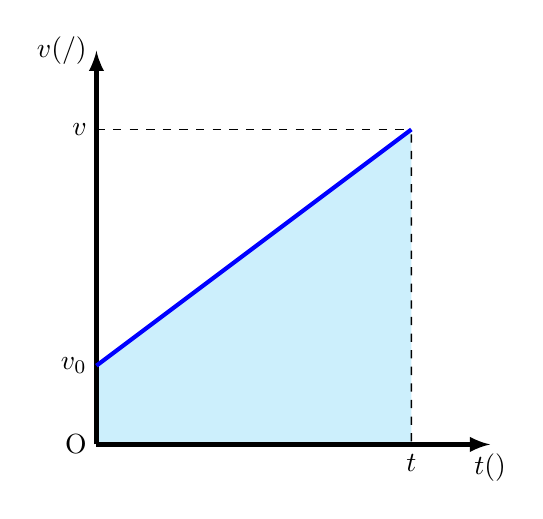
\begin{tikzpicture}  
					\coordinate (O) at(0,0);
					\coordinate (x) at(5,0);
					\coordinate (y) at(0,5);
					\coordinate (v0) at(0,1);
					\coordinate (v1) at(0,1.75);
					\coordinate (v2) at(0,4);
					\coordinate (B) at(4,4);
					\coordinate (A) at(1,1.75);
					\coordinate (C) at(4,0);
					\coordinate (D) at(1,0);
					\fill[cyan, opacity=0.2] (v0)--(B)--(C)--(O)--(v0);
					\draw[line width=0.5pt,black, dashed] (v0)--(B)--(C)--(O)--(v0);
					\draw[line width=0.5pt, dashed] (v2)--(B);
					\draw[-latex, line width=1.5pt] (O)--(x);
					\draw[-latex, line width=1.5pt] (O)--(y);
					\draw[blue, line width=1.5pt] (v0)--(B);
					\node[below] at(x) {$\xsi{t}{\left(\second\right)}$};
					\node[left] at(y) {$\xsi{v}{(\meter/\second)}$};
					\node[left] at(v0) {$v_0$};
					\node[left] at(0,4) {$v$};
					\node[left] at(O) {O};
					\node[below] at (C) {$t$};
				\end{tikzpicture}
			\end{center}
		}\\
		\multicolumn{2}{|L{17cm}|}{\dotfill}\\
		\multicolumn{2}{|L{17cm}|}{\dotfill}\\
		\multicolumn{2}{|L{17cm}|}{\dotfill}\\
		\multicolumn{2}{|L{17cm}|}{\dotfill}\\
		\hline
	\end{longtable}
\end{center}
\textbf{* Bài tập}\\
\textbf{BÀI TẬP TRẮC NGHIỆM}
\Opensolutionfile{ans}[ans/BAI7-TN]
% ===================================================================
\begin{ex}
	Một xe máy đang đứng yên, sau đó khởi động và bắt đầu tăng tốc. Nếu chọn chiều dương cùng  chiều chuyển động của xe, nhận xét nào sau đây là đúng? 
	\choice
	{$a<0$, $v<0$}
	{$a>0$, $v<0$}
	{\True $a>0$, $v>0$}
	{$a<0$, $v>0$}
	\loigiai{}
\end{ex}
% ===================================================================
\begin{ex}
	Gia tốc là đại lượng
	\choice
	{\True vector, đặc trưng cho sự biến thiên nhanh hay chậm của vận tốc}
	{vô hướng, đặc trưng cho tính chất nhanh hay chậm của chuyển động}
	{vector, đặc trưng cho tính chất nhanh hay chậm của chuyển động}
	{vô hướng, đặc trưng cho tính sự biến thiên nhanh hay chậm của vận tốc}
	\loigiai{}
\end{ex}
% ===================================================================
\begin{ex}
	Công thức liên hệ giữa độ dịch chuyển, vận tốc và gia tốc của chuyển động nhanh dần đều là
	\choice
	{$v^2-v^2_0=ad$}
	{\True $v^2-v^2_0=2ad$}
	{$v-v_0=2ad$}
	{$v^2_0-v^2=2ad$}
	\loigiai{}
\end{ex}
% ===================================================================
\begin{ex}
	Trong các phương trình mô tả vận tốc $v\ \left(\si{\meter/\second}\right)$ của vật theo thời gian $t\ \left(\si{\second}\right)$ dưới đây, phương trình nào mô tả chuyển động thẳng biến đổi đều?
	\choice
	{$v=7$}
	{$v=6t^2+2t-2$}
	{\True $v=5t-4$}
	{$v=6t^2-2$}
	\loigiai{}
\end{ex}
% ===================================================================
\begin{ex}
	Cho các đồ thị độ dịch chuyển - thời gian $\left(d-t\right)$ và vận tốc - thời gian $\left(v-t\right)$ như hình bên dưới. Đồ thị ứng với chuyển động thẳng biến đổi đều là
	\begin{center}
		\begin{tabular}{M{4cm}M{4cm}M{4cm}M{4cm}}
			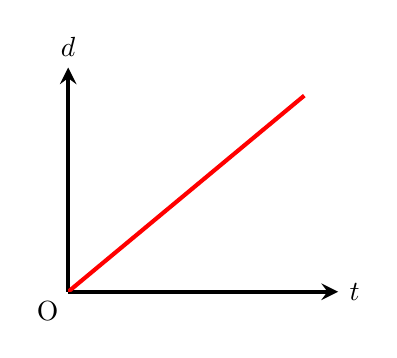
\begin{tikzpicture}  
				\begin{axis}[  ultra thick,scale=0.5,
					xmin=0,  
					xmax=4,  
					ymin=0,  
					ymax=4, 
					samples=300,
					yticklabels=\empty,
					xticklabels=\empty,
					xtick=\empty,
					ytick=\empty,
					axis lines=center, 
					xlabel=$t$, 		ylabel=$d$,
					every axis y label/.style={at=(current axis.above origin),anchor=south},  
					every axis x label/.style={at=(current axis.right of origin),anchor=west},  ]
					\addplot [line width=1.5pt, red, smooth, domain=0:3.5] {x};  
					\coordinate (O) at (0,0);
				\end{axis}  
				\node[below left] at (O) {O};
			\end{tikzpicture}&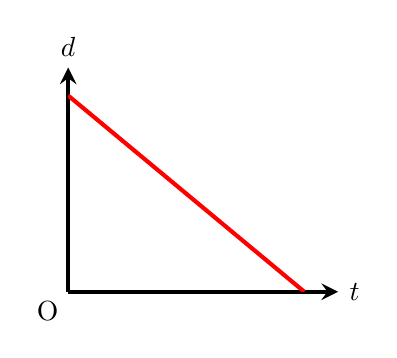
\begin{tikzpicture}  
				\begin{axis}[  ultra thick,scale=0.5,
					xmin=0,  
					xmax=4,  
					ymin=0,  
					ymax=4, 
					samples=300,
					yticklabels=\empty,
					xticklabels=\empty,
					xtick=\empty,
					ytick=\empty,
					axis lines=center, 
					xlabel=$t$, 		ylabel=$d$,
					every axis y label/.style={at=(current axis.above origin),anchor=south},  
					every axis x label/.style={at=(current axis.right of origin),anchor=west},  ]
					\addplot [line width=1.5pt, red, smooth, domain=0:3.5] {3.5-x};  
					\coordinate (O) at (0,0);
				\end{axis}  
				\node[below left] at (O) {O};
			\end{tikzpicture}&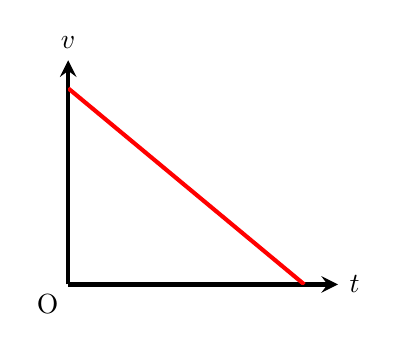
\begin{tikzpicture}  
				\begin{axis}[  ultra thick,scale=0.5,
					xmin=0,  
					xmax=4,  
					ymin=0,  
					ymax=4, 
					samples=300,
					yticklabels=\empty,
					xticklabels=\empty,
					xtick=\empty,
					ytick=\empty,
					axis lines=center, 
					xlabel=$t$, 		ylabel=$v$,
					every axis y label/.style={at=(current axis.above origin),anchor=south},  
					every axis x label/.style={at=(current axis.right of origin),anchor=west},  ]
					\addplot [line width=1.5pt, red, smooth, domain=0:3.5] {3.5-x};  
					\coordinate (O) at (0,0);
				\end{axis}  
				\node[below left] at (O) {O};
			\end{tikzpicture}&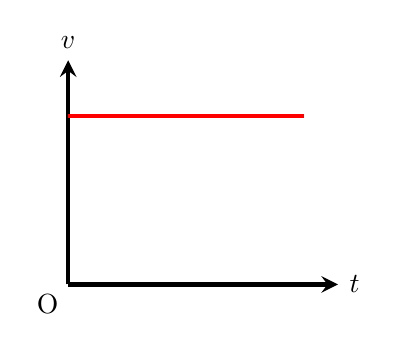
\begin{tikzpicture}  
				\begin{axis}[  ultra thick,scale=0.5,
					xmin=0,  
					xmax=4,  
					ymin=0,  
					ymax=4, 
					samples=300,
					yticklabels=\empty,
					xticklabels=\empty,
					xtick=\empty,
					ytick=\empty,
					axis lines=center, 
					xlabel=$t$, 		ylabel=$v$,
					every axis y label/.style={at=(current axis.above origin),anchor=south},  
					every axis x label/.style={at=(current axis.right of origin),anchor=west},  ]
					\addplot [line width=1.5pt, red, smooth, domain=0:3.5] {3};  
					\coordinate (O) at (0,0);
				\end{axis}  
				\node[below left] at (O) {O};
			\end{tikzpicture}\\
			Hình 1&Hình 2&Hình 3&Hình 4
		\end{tabular}
	\end{center}	
	\choice
	{Hình 1 và Hình 4}
	{Hình 2 và Hình 3}
	{\True Hình 3}
	{Hình 1}
	\loigiai{}
\end{ex}
% ===================================================================
\begin{ex}
	Chọn phát biểu \textbf{sai}.
	\choice
	{Gia tốc của vật chuyển động thẳng biến đổi đều có độ lớn không đổi}
	{\True Trong chuyển động thẳng biến đổi đều, quãng đường vật đi được trong những khoảng thời gian bằng nhau thì bằng nhau}
	{Vận tốc tức thời của vật chuyển động thẳng biến đổi đều có độ lớn tăng hoặc giảm đều theo thời gian}
	{Vectơ gia tốc của vật chuyển động thẳng biến đổi đều có thể cùng chiều hoặc ngược chiều với vectơ vận tốc}
	\loigiai{}
\end{ex}
% ===================================================================
\begin{ex}
	Một ô tô đang chạy với tốc độ $\SI{72}{\kilo\meter/\hour}$ thì hãm phanh, chạy chậm dần đều sau $\SI{10}{\second}$ tốc độ giảm còn $\SI{10}{\meter/\second}$. Thời gian từ lúc hãm phanh đến lúc dừng lại là
	\choice
	{$\SI{30}{\second}$}
	{\True $\SI{20}{\second}$}
	{$\SI{12}{\second}$}
	{$\SI{40}{\second}$}
	\loigiai{}
\end{ex}
% ===================================================================
\begin{ex}
	Trong chuyển động thẳng nhanh dần đều	
	\choice
	{$a<0$}
	{\True $v\cdot a>0$}
	{$ a>0$}
	{$v\cdot a<0$}
	\loigiai{}
\end{ex}
% ===================================================================
\begin{ex}
	Một ô tô đang chạy với tốc độ $\SI{12}{\meter/\second}$ trên một đoạn đường thẳng thì người lái xe tăng
	ga cho ôtô chạy nhanh dần đều. Sau $\SI{15}{\second}$ ôtô đạt tốc độ $\SI{15}{\meter/\second}$. Quãng đường của ô tô
	đi được sau $\SI{5}{\second}$ kể từ khi tăng ga là	
	\choice
	{$\SI{72.5}{\meter}$}
	{$\SI{65}{\meter}$}
	{$\SI{57.5}{\meter}$}
	{\True $\SI{62.5}{\meter}$}
	\loigiai{}
\end{ex}
% ===================================================================
\begin{ex}
	Một đoàn tàu đang đứng yên  thì bắt đầu tăng tốc chuyển động thẳng nhanh dần đều. Trong khoảng thời gian tăng tốc từ $\SI{21.6}{\kilo\meter/\hour}$ đến $\SI{36}{\kilo\meter/\hour}$, tàu đi được $\SI{64}{\meter}$. Gia tốc của tàu và quãng đường tàu đi được kể từ lúc bắt đầu chuyển động đến khi đạt tốc độ $\SI{36}{\kilo\meter/\hour}$ là
	\choice
	{$a=\SI{-0.7}{\meter/\second^2}$, $s=\SI{200}{\meter}$}
	{$a=\SI{-0.5}{\meter/\second^2}$, $s=\SI{110}{\meter}$}
	{\True $a=\SI{0.5}{\meter/\second^2}$, $s=\SI{100}{\meter}$}
	{$a=\SI{-0.5}{\meter/\second^2}$, $s=\SI{100}{\meter}$}
	\loigiai{}
\end{ex}

% ===================================================================
\begin{ex}
	Hình bên mô tả đồ thị $\left(v-t\right)$ của bốn xe ô tô A, B, C, D. Nhận định nào sau đây là đúng?
	\begin{center}
		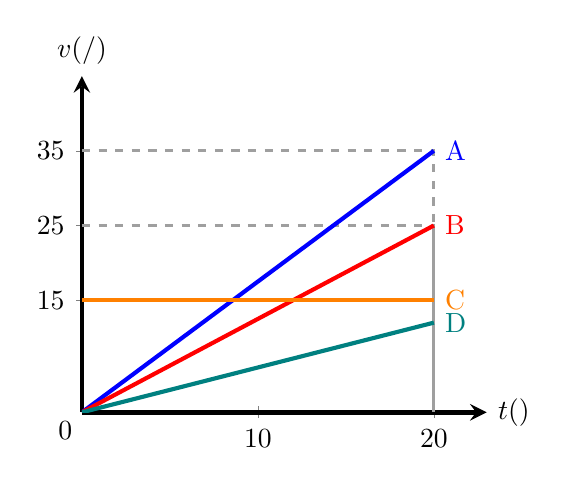
\begin{tikzpicture}  
			\begin{axis}[  ultra thick,scale=0.75,
				xmin=0,  
				xmax=23,  
				xtick={0,10,20},
				ytick={0,15,25,35},
				ymin=0,  
				ymax=45, 
				samples=300,
				axis lines=center, 
				xlabel=$\xsi{t}{\left(\si{\second}\right)}$, 		ylabel=$\xsi{v}{\left(\si{\meter/\second}\right)}$,
				every axis y label/.style={at=(current axis.above origin),anchor=south},  
				every axis x label/.style={at=(current axis.right of origin),anchor=west},  ]
				\draw[dashed, line width=1pt, gray!75!white] (axis cs: 0,35)--(axis cs: 20,35)--(axis cs: 20,0);
				\draw[dashed, line width=1pt, gray!75!white] (axis cs: 0,25)--(axis cs: 20,25)--(axis cs: 20,0);
				\addplot [line width=1.5pt, blue, smooth, domain=0:20] {1.75*x} node[right] {A};
				\addplot [line width=1.5pt, red, smooth, domain=0:20] {1.25*x} node[right] {B}; 
				\addplot [line width=1.5pt,teal , smooth, domain=0:20] {0.6*x} node[right] {D}; 
				\addplot [line width=1.5pt, orange, smooth, domain=0:20] {15} node[right] {C};
				\coordinate (O) at (0,0);
			\end{axis}  
			\node[below left] at (O) {0};
		\end{tikzpicture}
	\end{center}	
	\choice
	{\True Xe C chuyển động đều, còn các xe còn lại là chuyển động biến đổi đều}
	{Chỉ có xe A và B chuyển động biến đồi đều, xe C chuyển động đều}
	{Gia tốc xe A có độ lớn nhỏ hơn gia tốc xe D}
	{Xe D chuyển động biến đổi đều, xe C chuyển động đều}
	\loigiai{}
\end{ex}
% ===================================================================
\begin{ex}
	Một vật chuyển động dọc theo trục $Ox$ có phương trình chuyển động $x=3-4t+2t^2\ \left(\si{\meter};\si{\second}\right)$. Biểu thức vận tốc của vật theo thời gian là
	\choice
	{$v=\xsi{2\left(t-2\right)}{\meter/\second}$}
	{$v=\xsi{2\left(t+2\right)}{\meter/\second}$}
	{\True $v=\xsi{4\left(t-1\right)}{\meter/\second}$}
	{$v=\xsi{2\left(t-1\right)}{\meter/\second}$}
	\loigiai{}
\end{ex}
% ===================================================================
\begin{ex}
	Một vật chuyển động dọc theo trục $Ox$ có phương trình chuyển động $x=10t+5t^2\ \left(\si{\meter}; \si{\second}\right)$. Vận tốc của vật tại thời điểm $t=\SI{2}{\second}$ là	
	\choice
	{$\SI{40}{\meter/\second}$}
	{$\SI{20}{\meter/\second}$}
	{\True $\SI{30}{\meter/\second}$}
	{$\SI{26}{\meter/\second}$}
	\loigiai{}
\end{ex}
% ===================================================================
\begin{ex}
	Phương trình chuyển động của một vật trên trục $Ox$ có dạng: $x=-2t^2+15t+10$.	Trong đó $t$ tính bằng giây, $x$ tính bằng mét. Vật này chuyển động
	\choice
	{nhanh dần đều rồi chậm dần đều theo chiều dương của trục $Ox$}
	{chậm dần đều rồi nhanh dần đều theo chiều âm của trục $Ox$}
	{nhanh dần đều rồi chậm dần đều theo chiều âm của trục $Ox$}
	{\True chậm dần đều theo chiều dương rồi nhanh dần đều theo chiều âm của trục $Ox$}
	\loigiai{}
\end{ex}
% ===================================================================
\begin{ex}
	\immini{Đồ thị vận tốc - thời gian của một vật chuyển động thẳng biến đổi trong 5 giây đầu tiên được cho như hình vẽ bên. Kết luận nào sau đây là đúng?
		\choice
		{\True Vật chuyển động chậm dần đều theo chiều âm với gia tốc $\SI{2}{\meter/\second^2}$}
		{Vật chuyển động thẳng đều theo chiều dương}
		{Vật chuyển động nhanh dần đều theo chiều dương với gia tốc $\SI{2}{\meter/\second^2}$}
		{Vật chuyển động nhanh dần đều theo chiều âm với gia tốc $\SI{-2}{\meter/\second^2}$}
		\loigiai{}}
	{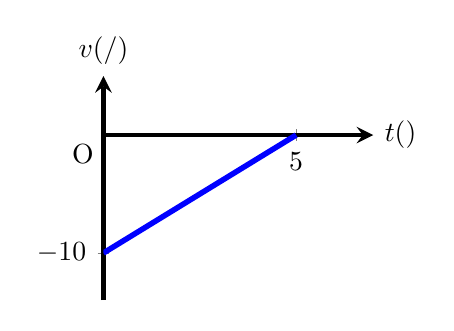
\begin{tikzpicture}  
			\begin{axis}[  ultra thick,scale=0.5,
				xmin=0,  
				xmax=7,  
				xtick={0,5},
				ytick={-10,0},
				ymin=-14,  
				ymax=5, 
				samples=300,
				axis lines=center, 
				xlabel=$\xsi{t}{\left(\si{\second}\right)}$, 		ylabel=$\xsi{v}{\left(\si{\meter/\second}\right)}$,
				every axis y label/.style={at=(current axis.above origin),anchor=south},  
				every axis x label/.style={at=(current axis.right of origin),anchor=west},  ]
				\addplot [line width=2pt, blue, smooth, domain=0:5] {-10+2*x};  
				\coordinate (O) at (axis cs: 0,0);
			\end{axis}  
			\node[below left] at (O) {O};
	\end{tikzpicture}}
\end{ex}
% ===================================================================
\begin{ex}
	Một vật chuyển động thẳng có đồ thị vận tốc theo thời gian như hình vẽ. Quãng đường vật đi được trong giai đoạn chậm dần đều là
	\begin{center}
		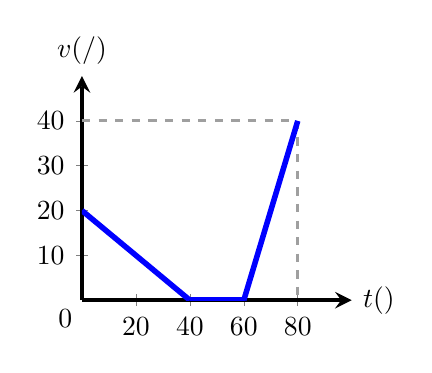
\begin{tikzpicture}  
			\begin{axis}[  ultra thick,scale=0.5,
				xmin=0,  
				xmax=100,  
				xtick={0,20,...,80},
				ytick={0,10,...,40},
				minor x tick num=0,
				minor y tick num=0,
				ymin=0,  
				ymax=50, 
				samples=300,
				axis lines=center, 
				xlabel=$\xsi{t}{\left(\si{\second}\right)}$, 		ylabel=$\xsi{v}{\left(\si{\meter/\second}\right)}$,
				every axis y label/.style={at=(current axis.above origin),anchor=south},  
				every axis x label/.style={at=(current axis.right of origin),anchor=west},  ]
				\draw[dashed, line width=1pt, gray!75!white] (axis cs: 0,40)--(axis cs: 80,40)--(axis cs: 80,0);
				\addplot [line width=2pt, blue, smooth, domain=0:40] {20-0.5*x};  
				\addplot [line width=2pt, blue, smooth, domain=40:60] {0}; 
				\addplot [line width=2pt, blue, smooth, domain=60:80] {2*(x-60)}; 
				\coordinate (O) at (0,0);
			\end{axis}  
			\node[below left] at (O) {0};
		\end{tikzpicture}
	\end{center}
	\choice
	{$\SI{600}{\meter}$}
	{$\SI{800}{\meter}$}
	{$\SI{200}{\meter}$}
	{\True $\SI{400}{\meter}$}
	\loigiai{}
\end{ex}
% ===================================================================
\begin{ex}
	Quan sát đồ thị $\left(v-t\right)$ như hình bên dưới của một vật đang chuyển động thẳng và cho biết quãng đường vật đi được trong khoảng thời gian nào lớn nhất?
	\begin{center}
		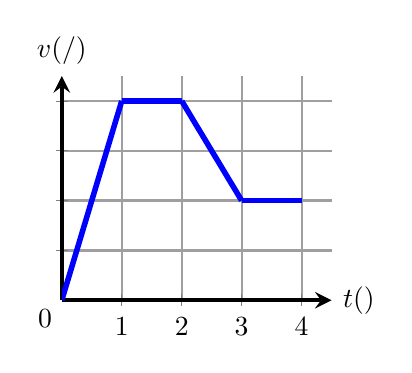
\begin{tikzpicture}  
			\begin{axis}[  ultra thick,scale=0.5,
				xmin=0,  
				xmax=4.5,  
				xtick={0,1,...,4},
				ytick={0,1,...,4},
				minor x tick num=0,
				minor y tick num=0,
				ymin=0,  
				ymax=4.5, 
				samples=300,
				yticklabels=\empty,
				axis lines=center, 
				grid style={step=1, line width =0.4pt, color=gray!40!white},
				grid=both, %giới hạn ô lưới
				major grid style={line width=0.8pt,gray!75!white},
				xlabel=$\xsi{t}{\left(\si{\second}\right)}$, 		ylabel=$\xsi{v}{\left(\si{\meter/\second}\right)}$,
				every axis y label/.style={at=(current axis.above origin),anchor=south},  
				every axis x label/.style={at=(current axis.right of origin),anchor=west},  ]
				\addplot [line width=2pt, blue, smooth, domain=0:1] {4*x};  
				\addplot [line width=2pt, blue, smooth, domain=1:2] {4}; 
				\addplot [line width=2pt, blue, smooth, domain=2:3] {4-2*(x-2)}; 
				\addplot [line width=2pt, blue, smooth, domain=3:4] {2}; 
				\coordinate (O) at (0,0);
			\end{axis}  
			\node[below left] at (O) {0};
		\end{tikzpicture}
	\end{center}
	\choice
	{Trong khoảng thời gian từ $\SI{0}{\second}$ đến $\SI{1}{\second}$}
	{\True Trong khoảng thời gian từ $\SI{1}{\second}$ đến $\SI{2}{\second}$}
	{Trong khoảng thời gian từ $\SI{2}{\second}$ đến $\SI{3}{\second}$}
	{Trong khoảng thời gian từ $\SI{3}{\second}$ đến $\SI{4}{\second}$}
	\loigiai{}
\end{ex}
% ===================================================================
\begin{ex}
	Đồ thị vận tốc - thời gian của một vật chuyển động thẳng biến đổi đều được cho như hình vẽ bên. Biết rằng $v_1+v_2=\SI{15}{\meter/\second}$ và $t_2-t_1=\SI{6}{\second}$. Quãng đường vật đi được trong khoảng thời gian từ $t_1$ đến $t_2$ là
	\begin{center}
		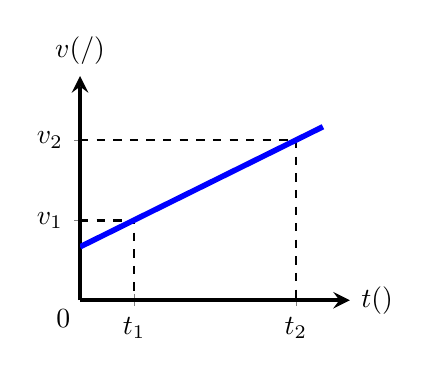
\begin{tikzpicture}  
			\begin{axis}[  ultra thick,scale=0.5,
				xmin=0,  
				xmax=10,  
				xtick={0,2,8},
				ytick={0,5,10},
				ymin=0,  
				ymax=14, 
				samples=300,
				yticklabels={0,$v_1$,$v_2$},
				xticklabels={0,$t_1$,$t_2$},
				axis lines=center, 
				xlabel=$\xsi{t}{\left(\si{\second}\right)}$, 		ylabel=$\xsi{v}{\left(\si{\meter/\second}\right)}$,
				every axis y label/.style={at=(current axis.above origin),anchor=south},  
				every axis x label/.style={at=(current axis.right of origin),anchor=west},  ]
				\draw[dashed, line width=1pt] (axis cs: 0,5)--(axis cs: 2,5)--(axis cs: 2,0);
				\draw[dashed, line width=1pt] (axis cs: 0,10)--(axis cs: 8,10)--(axis cs: 8,0);
				\addplot [line width=2pt, blue, smooth, domain=0:9] {10/3+5*x/6};  
				\coordinate (O) at (0,0);
			\end{axis}  
			\node[below left] at (O) {0};
		\end{tikzpicture}
	\end{center}	
	\choice
	{$\SI{90}{\meter}$}
	{\True $\SI{45}{\meter}$}
	{$\SI{9}{\meter}$}
	{$\SI{540}{\meter}$}
	\loigiai{}
\end{ex}
% ===================================================================
\begin{ex}
	Một xe máy chạy đều trên một con đường thẳng với tốc độ $\SI{20}{\meter/\second}$ (vượt quá tốc độ) thì bị cảnh sát giao thông phát hiện. Chỉ sau $\SI{2}{\second}$ khi xe máy đi qua một cảnh sát, anh cảnh sát này bắt đầu đuổi theo với gia tốc không đổi và bằng $\SI{1.05}{\meter/\second^2}$. Thời điểm và vị trí anh cảnh sát đuổi kịp xe máy là
	\choice
	{\True sau $\SI{40}{\second}$ kể từ lúc anh cảnh sát xuất phát, cách vị trí xuất phát $\SI{840}{\meter}$}
	{sau $\SI{42}{\second}$ kể từ lúc anh cảnh sát xuất phát, cách vị trí xuất phát $\SI{840}{\meter}$}
	{sau $\SI{38}{\second}$ kể từ lúc anh cảnh sát xuất phát, cách vị trí xuất phát $\SI{760}{\meter}$}
	{sau $\SI{36}{\second}$ kể từ lúc anh cảnh sát xuất phát, cách vị trí xuất phát $\SI{760}{\meter}$}
	\loigiai{}
\end{ex}
% ===================================================================
\begin{ex}
	Hai xe A và B chuyển động cùng nhau vào hầm Thủ Thiêm dài $\SI{1490}{\meter}$. Xe A chuyển động với tốc độ ban đầu trước khi vào hầm là $\SI{60}{\kilo\meter/\hour}$ và chuyển động chậm dần đều với độ lớn gia tốc $\SI{144}{\kilo\meter/\hour^2}$, xe B chuyển động chậm dần đều với gia tốc $\SI{120}{\kilo\meter/\hour^2}$	từ lúc bắt đầu chạy vào hầm với tốc độ $\SI{55}{\kilo\meter/\hour}$. Nhận định nào sau đây là đúng về thời gian chuyển động của hai xe trong hầm?
	\choice
	{Hai xe đi hết hầm Thủ Thiêm cùng một khoảng thời gian}
	{Xe B ra khỏi hầm trước xe A}
	{\True Xe A ra khỏi hầm trước xe B}
	{Dữ liệu bài toán không đủ kết luận}
	\loigiai{}
\end{ex}
\Closesolutionfile{ans}
\textbf{BÀI TẬP TỰ LUẬN}
\Opensolutionfile{ans}[ans/BAI7-TL]
\setcounter{ex}{0}
% ======================================================================
\begin{ex}
	Quan sát đồ thị $\left(v-t\right)$ mô tả chuyển động thẳng của tàu hỏa trong hình bên dưới và trả lời các câu hỏi:
	\begin{center}
		\includegraphics[scale=0.4]{figs/BAI7-1}
	\end{center}
	\begin{enumerate}[label=\alph*)]
		\item Tại thời điểm nào, vận tôc tàu hỏa có giá trị lớn nhất?
		\item Vận tốc tàu hỏa không đổi trong khoảng thời gian nào?
		\item Tàu chuyển động thẳng nhanh dần đều trong khoảng thời gian nào?
	\end{enumerate}
	\loigiai{}
\end{ex}

% ======================================================================
\begin{ex}
	Đồ thị vận tốc $(v)$ – thời gian $(t)$ của một vật chuyển động thẳng được cho như hình bên. Xác định quãng đường vật đi được trong 6 giây đầu tiên và 6 giây cuối cùng của chuyển động.
	\begin{center}
		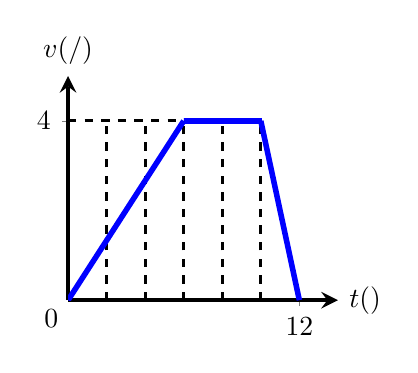
\begin{tikzpicture}  
			\begin{axis}[  ultra thick,scale=0.5,
				xmin=0,  
				xmax=14,  
				xtick={0,12},
				ytick={0,4},
				ymin=0,  
				ymax=5, 
				samples=300,
				axis lines=center,
				xlabel=$\xsi{t}{\left(\si{\second}\right)}$, 		ylabel=$\xsi{v}{\left(\si{\meter/\second}\right)}$,
				every axis y label/.style={at=(current axis.above origin),anchor=south},  
				every axis x label/.style={at=(current axis.right of origin),anchor=west},  ]
				\foreach \i in {2,4,...,10}{
					\edef\temp{\noexpand\draw[dashed, line width=1pt] (axis cs: \i,0)--(axis cs: \i,4);}
					\temp
				}
				\draw[dashed, line width=1pt] (axis cs: 0,4)--(axis cs: 10,4);
				\draw[dashed, line width=1pt] (axis cs: 0,40)--(axis cs: 80,40)--(axis cs: 80,0);
				\addplot [line width=2pt, blue, smooth, domain=0:6] {2*x/3};  
				\addplot [line width=2pt, blue, smooth, domain=6:10] {4}; 
				\addplot [line width=2pt, blue, smooth, domain=10:12] {4-2*(x-10)}; 
				\coordinate (O) at (0,0);
			\end{axis}  
			\node[below left] at (O) {0};
		\end{tikzpicture}
	\end{center}
	\loigiai{}
\end{ex}
% ======================================================================
\begin{ex}
	Một người đạp xe trên đường thẳng với tốc độ $\SI{4}{\meter/\second}$, bóp thắng để giảm tốc với gia tốc có độ lớn không đổi là $\SI{0.5}{\meter/\second^2}$. Xác định thời gian và quãng đường xe đi được từ khi bóp thắng đến khi dừng lại.
	\loigiai{}
\end{ex}
% ======================================================================
\begin{ex}
	Một ô tô chuyễn động chầm dần đều, trong $\SI{8.5}{\second}$ đi được quãng đường $\SI{40.0}{\meter}$ với vận tốc cuối cùng là $\SI{2.80}{\meter/\second}$.
	\begin{enumerate}[label=\alph*)]
		\item Tìm độ lớn vận tốc ban đầu của xe.
		\item Tìm gia tốc của xe.
	\end{enumerate}
	\loigiai{}
\end{ex}
% ======================================================================
\begin{ex}
	Tại hiện trường một vụ tai nạn trên đường quốc lộ ngoài đô thị, cảnh sát phát hiện vết trượt kéo dài $\SI{50}{\meter}$. Qua các đo đạc trên mặt đường, cảnh sát kết luận gia tốc của ô tô trong quá trình giảm tốc có độ lớn $\SI{6.5}{\meter/\second^2}$. Nếu tốc độ giới hạn trên làn đường được quy định là $\SI{80}{\kilo\meter/\hour}$ thì ô tô này có vượt quá tốc độ cho phép không? Giả sử trong quá trình giảm tốc, ô tô chuyển động chậm dần đều.
	\loigiai{}
\end{ex}
% ======================================================================
\begin{ex}
	Một ô tô đang đi trên đường thẳng với tốc độ $v$ thì trước mặt ô tô đột ngột xuất hiện một mối nguy hiểm. Trong khoảng thời gian từ khi mối nguy xuất hiện đến khi phanh hoạt động, ô tô chuyển động được quãng đường $\SI{29.3}{\meter}$. Khi phanh hoạt động làm bánh xe ngừng quay, các bánh xe của ô tô để lại vết trượt dài $\SI{12.8}{\meter}$ trên đường, như minh hoạ trong hình bên dưới.
	\begin{center}
		\includegraphics[width=0.5\linewidth]{figs/BAI7-2}
	\end{center}
	Người ta ước tính rằng trong quá trình trượt, ô tô giảm tốc với gia tốc có độ lớn là $\SI{8.33}{\meter/\second^2}$. Xác định:
	\begin{enumerate}[label=\alph*)]
		\item Tốc độ $v$ của ô tô trước khi hãm phanh.
		\item Khoảng thời gian từ khi nguy hiểm xuất hiện đến khi phanh hoạt động.
	\end{enumerate}
	\loigiai{}
\end{ex}
% ======================================================================
\begin{ex}
	Một ô tô khi hãm phanh có thể có gia tốc $\SI{3}{\meter/\second^2}$. Hỏi khi ô tô đang chạy với vận tốc là $\SI{72}{\kilo\meter/\hour}$ thì phải hãm phanh cách vật cản là bao nhiêu mét để không đâm vào vật cản? Thời gian hãm phanh là bao nhiêu?
	\loigiai{}
\end{ex}
% ======================================================================
\begin{ex}
	Một xe đạp đang đi với tốc độ $\SI{2}{\meter/\second}$ thì xuống dốc chuyển động nhanh dần đều với độ lớn gia tốc $\SI{0.2}{\meter/\second^2}$. Cùng lúc đó, một ô tô đang chạy với tốc độ $\SI{20}{\meter/\second}$ lên dốc,
	chuyển động chậm dần đều với độ lớn gia tốc $\SI{0.4}{\meter/\second^2}$. Xác định vị trí hai xe gặp nhau trên dốc. Biết dốc dài $\SI{570}{\meter}$.
	\loigiai{$\SI{420}{\meter}$}
\end{ex}
% ======================================================================
\begin{ex}
	\immini{
		Hai vật A và B chuyển động cùng chiều trên đường thẳng (theo hướng từ A sang B) có đồ thị vận tốc - thời gian vẽ ở hình vẽ bên. Biết ban đầu hai vật cách nhau $\SI{78}{\meter}$.
		\begin{enumerate}[label=\alph*)]
			\item Hai vật có cùng vận tốc ở thời điểm nào?
			\item Viết phương trình chuyển động của mỗi vật.
			\item Xác định vị trí gặp nhau của hai vật.
		\end{enumerate}
	}
	{
		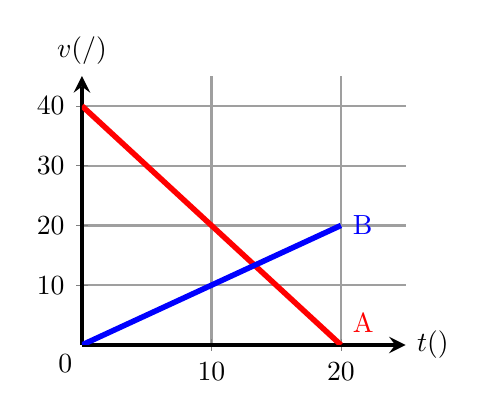
\begin{tikzpicture}  
			\begin{axis}[  ultra thick,scale=0.6,
				xmin=0,  
				xmax=25,  
				xtick={0,10,20},
				ytick={0,10,...,40},
				minor x tick num=0,
				minor y tick num=0,
				ymin=0,  
				ymax=45, 
				samples=300,
				axis lines=center, 
				grid style={step=1, line width =0.4pt, color=gray!40!white},
				grid=both, %giới hạn ô lưới
				major grid style={line width=0.8pt,gray!75!white},
				xlabel=$\xsi{t}{\left(\si{\second}\right)}$, 		ylabel=$\xsi{v}{\left(\si{\meter/\second}\right)}$,
				every axis y label/.style={at=(current axis.above origin),anchor=south},  
				every axis x label/.style={at=(current axis.right of origin),anchor=west},  ]
				\addplot [line width=2pt, red, smooth, domain=0:20] {40-2*x} node[above right] {A}; 
				\addplot [line width=2pt, blue, smooth, domain=0:20] {x} node[right] {B};  
				\coordinate (O) at (axis cs: 0,0);
			\end{axis}  
			\node[below left] at (O) {0};
		\end{tikzpicture}
	}
	\loigiai{}
\end{ex}
% ======================================================================
\begin{ex}
	Một người đứng ở sân ga nhìn ngang đầu toa tàu thứ nhất của một đoàn tàu bắt đầu chuyển bánh. Thời gian toa thứ nhất qua trước mặt người ấy là $t_1=\SI{6}{\second}$. Hỏi toa thứ 7 qua trước mặt người ấy trong bao lâu? Biết rằng đoàn tàu chuyển động thẳng nhanh dần đều, chiều dài các toa bằng nhau và khoảng hở giữa 2 toa là không đáng kể.
	\loigiai{}
\end{ex}
\Closesolutionfile{ans}